\documentclass[../masterarbeit.tex]{subfiles}
\begin{document}


\section{Results}
\begin{figure}[h]
    \centering
    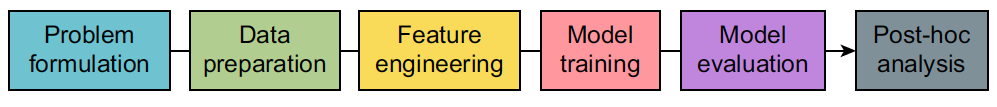
\includegraphics[scale=0.4]{supervised_machine_learning_pipeline.png}
    \source{\autocite[]{VIEIRA202021}}
    \caption{The six steps of the supervised machine learning pipeline.}
    \end{figure} 
This chapter describes the actual study including the results. The study is divided into different steps. The supervised machine learning pipeline presented in Figure 13 shows the six steps of a study using supervised machine learning models. It starts with the step of defining the Problem or Goal of the study. 
The problem to be solved in context of this master thesis is to predict snow avalanches with meteorological dan snow pack related data for topographical defined mountain slopes and answer the two Research questions mentioned in chapter 1. The problem falls into the category of binary classifications problems, since it has the two predictive values "Avalanche" and "Non-avlanache".
The second phase is about data preparation. In the case of this work it starts with information about the data owner and the study area. Followed by the composition of the data set as well as its data preprocessing. Every features in the resulting data set is described. 
The feature selection process, which in this case consists of two steps, is also discussed. In the first step, a decision tree is used to select a number of meteorological features for which additional columns for data from the past days are added to the data set. In the second step, a genetic algorithm is executed on the three machine learning models Logistic Regression, LDA and SVM to calculate the optimal feature subset for each algorithm. 
The training phase of the three supervised classification machine learning models is described together with the model evaluations in section 4.3, because they represent the results of the model training phase.










\subfile{sections/data.tex}

\clearpage
\newpage
\subfile{sections/feature_selection.tex}
    
  
\clearpage
\newpage

  
\clearpage
\newpage
\subfile{sections/model_training_evaluation.tex}







\end{document}